\newpage
\chapter{Theorie}
%\section{Theorie}
\section{Elementare Strahler}\label{sec:ElementareStrahler}
Es gibt zwei elementare Strahler. Der eine stellt eine E Feld Antenne dar, der andere eine H Feld Antenne. Die beiden elementaren Strahler lassen sich nicht praktisch fertigen. Sie dienen nur für theoretische Überlegungen. Sie bilden jedoch die Grundlage sämtlicher realen Antennen.
\section{Hertzscher Dipol}
Ein elektrisch kurzer Linearstrahler kann als konzentriertes Element betrachtet werden. Auf seiner gesamten Länge kann ein Strom mit der  Amplitude $I$ und eine räumlich konstante Stromverteilung, die zeitlich sinusförmig schwingt, angenommen werden. Es stellt sich ein kurzer Stromfaden ein, dessen Stromrichtung von der Polarisierung der Dipole abhängt und somit mit $\omega $ die Richtung wechselt. 
Der Hertzsche Dipol bildet den elementaren Elektrischen Dipol. Man kann ihn sich als eine sehr kurze Stabantenne vorstellen. Der Betrag des Dipolmoments \textit{p(t)} eines Hertzschen Dipols ist als $\textit{p}=Q\textit{d}l$ in (\ref{Dipolmoment}) beschrieben \cite{Emant}. Der Scheitelwert $\hat{i}$ des Stromes  schwingt mit der Kreisfrequenz  $\omega$.

\begin{equation}\label{Dipolmoment}
p(t)=pe^{j\omega t} = Q dl e^{j\omega t} = \frac{\hat{i} dl}{j\omega }e^{j\omega t}
\end{equation}
Ist ein Hertzscher Dipol unendlich dünn und in einem xyz Koordinatensystem im Ursprung und in die z Richtung ausgerichtet, so bildet sich ein E Feld vom positiven  zum negativen Ladungspunkt. Die Potentiale der Ladungspunkte oszillieren mit $\omega$. Die Ausrichtung der E Feldlinien wechselt bei jeder Schwingung ihre Richtung. Im Nahfeld dominiert das E Feld. Mit wachsendem Abstand von dem Strahler, sind das E Feld und das H Feld senkrecht zueinander und in Phase. Dabei können das E und H Feld als ebene Welle betrachtet werden. Die allgemeine Formel für die Feldverteilung im Kugelkoordinaten System lautet \cite{elliott1981antenna}:
%\begin{center}
%\begin{minipage}{\linewidth}
%\centering
%\includegraphics{\conten\bilder\Herz_Dipol_EMANT_S37.pdf}%
%\captionof{figure}[kurze Bildunterschrift]{Bildunterschrift}%
%\end{minipage}
%\end{center}



%\begin{figure}[htbp]
%	\centering
%		\includegraphics[width=8cm]{content/Bilder/Z0_Grafik.png}
%	\caption{Wellenimpdedanz Z0}%
%	\label{Z0_Grafik}
%\end{figure}




\begin{equation}
E_r= \frac{I dl}{2\pi}   e^{-jkR} \left( \frac{n}{R^{2}}  + \frac{1}{j\omega \epsilon R^{3}}\right) cos(\theta)
\end{equation}

\begin{equation}
E_\theta= \frac{I dl}{4\pi}   e^{-jkR} \left( \frac{j\omega \mu}{R}  + \frac{n}{R^{2}}+ \frac{1}{j\omega \epsilon R^{3}}\right) sin(\theta)
\end{equation}

\begin{equation}
H_\varphi= \frac{I dl}{4\pi}   e^{-jkR} \left( \frac{jk}{R}  + \frac{n}{R^{2}}\right) sin(\theta)
\end{equation}

\begin{figure}[!ht]
	\centering
	\includegraphics[width=4cm]{content/bilder/HerzDipolEMANTS37.pdf}%
	\caption{Hertzscher Dipol mit dem Dipolmoment \textit{p(t)} \cite{Emant}}
	\label{HerzDipol}
\end{figure}


Mit wachsendem Abstand können einige Terme vernachlässigt werden. Alle Terme, in denen der Abstand R in höherer Potenz vorkommt, werden vereinfacht zu Null. Für das Fernfeld ergeben sich die folgenden Beschreibungen \cite{elliott1981antenna}:


\begin{equation}
E_r= 0
\end{equation}

\begin{equation}
E_\theta= \frac{I dl}{4\pi}   e^{-jkR} \left( \frac{j\omega \mu}{R}  \right) sin(\theta)
\end{equation}

\begin{equation}
H_\varphi= \frac{I dl}{4\pi}   e^{-jkR} \left( \frac{jk}{R} \right) sin(\theta)
\end{equation}
In weiter Ferne vom Elementaren Strahler sind die Feldanteile von $E_r$ soweit abgeklungen, dass sie als Null angenommen werden. Es bleibt ein E Feld Vektor und ein H Feld Vektor übrig. Vereinfacht können die beiden E und H Vektoren als phasengleich und senkrecht zueinander angenommen werden. Sie werden sich soweit im Raum ausbreiten, bis ihre gesamte Energie absorbiert ist. Das bedeutet, die Amplituden der E und H Vektoren werden Null.\\
Für alle Antennen, die eine lange und dünne Geometrie besitzen, wie zum Beispiel die Monopolantennen, die Dipolantennen oder die Faltdipole bildet der Hertzsche Dipol die Grundlage der Feldausbreitung. Die Ausdehnung des Elementaren Strahlers ist auf eine Länge der strahlenden Struktur von etwa $100\mu m$ beschränkt. Das bedeutet, der Gültigkeitsbereich der in dieser Arbeit gezeigten Formeln und Beschreibungen führen bis einer Frrequenz von 3 THz. Da die Wellenlänge $\lambda$ bei ca. 3 THz einer Länge von 100$\mu m$ entspricht.\\
Die Elektromagnetischen Felder eines Hertzschen Dipols werden oft in Kugelkoordinaten beschrieben. Jeder Punkt kann mit einem Vektor $\vec{r}$ mit dem Start Punkt im Ursprung beschrieben werden. Die Spitze des Vektor $\vec{r}$ kann in die xy Ebene projiziert werden. Der Winkel $\varphi$, gesprochen phi, liegt in der xy Ebene und startet bei der positiven x Achse. Er kann Werte von $\pm \pi$ erreichen und deckt somit $360^\circ$ ab. Der Winkel $\theta$, gesprochen theta, gibt die Neigung  des Vektors $\vec{r}$ zu der positiven z Achse an. Ein Vektor $\vec{r}$ ist in der Abbildung \ref{FerdVektor} gezeigt.




%%%%%%%%%%%%%%%%%%%%%%%%%%%%%%%%%%%
\begin{figure}[!ht]
\begin{center}
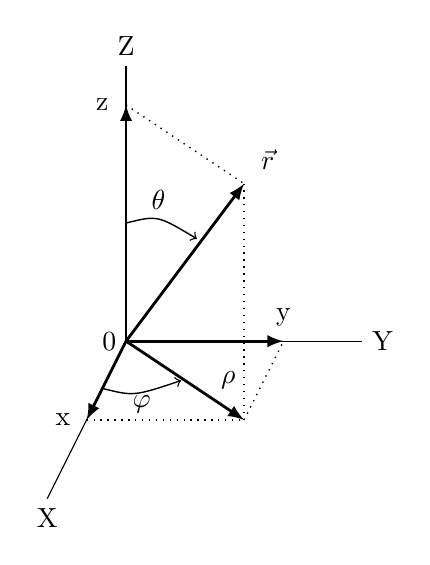
\begin{tikzpicture}
	\draw (4,4) -- (3,2) node[below] {X};%Fadenkreuz x
	\draw (4,4) node[left] {0} -- (7,4)node [right] {Y};%Fadenkreuz y
	\draw (4,4) -- (4,7.5) node[above] {Z};%Fadenkreuz z
	
	\draw[line width=1pt, ->, >=latex](4, 4)  -- (3.5, 3) node at (3.2, 3) {x};
	\draw[line width=1pt, ->, >=latex](4, 4)  -- (6, 4) node at (6, 4.3) {y};
	\draw[line width=1pt, ->, >=latex](4, 4)  -- (4, 7) node at (3.7, 7) {z};
	
	\draw[line width=0.5pt, style=dotted](3.5, 3) -- (5.5, 3);%Projektion y Rcihtung
	\draw[line width=0.5pt, style=dotted](5.5, 3) -- (6, 4);%Projektion x Rcihtung
	
	\draw[line width=1pt, ->, >=latex](4, 4)  -- (5.5, 3) node at (5.3, 3.5) {$\rho$};
	
	\draw[line width=1pt, ->, >=latex](4, 4)  -- (5.5, 6) node at (5.8, 6.3) {$\vec{r}$};
	
	\draw[line width=0.5pt, style=dotted](5.5, 3) -- (5.5, 6);%Projektion p zu \vec{r}
	\draw[line width=0.5pt, style=dotted](4, 7) -- (5.5, 6);%Projektion von z zur \vec{r}
	
	\coordinate (A) at (4, 5.5);
	\coordinate (B) at (4.9, 5.3);
	\coordinate (a) at (4.4, 5.6);
	\draw[line width=0.5pt, cap=round,->](A) .. controls (a) .. node[above] {$\theta$} (B);
	
	\coordinate (C) at (3.7, 3.4);
	\coordinate (D) at (4.7, 3.5);
	\coordinate (c) at (4.1, 3.3);
	\draw[line width=0.5pt, cap=round,->](C) .. controls (c) .. (D) node at (4.2, 3.2){$\varphi$};
\end{tikzpicture}
\end{center}
	\caption{Aufbau des Kugelkoordinatensystem}
	\label{FerdVektor}
\end{figure}

%%%%%%%%%%%%%%%%%%%%%%%%%%%%%%%%%%%%%%%%%%%%%%%%%%%%%%%%%%%%%%%%%%%

%%%%%%%%%%%%%%%%%%%%%%%%%%%%%%%%%%%%%%%%%%%%%%%%%%%%%%%%%%%%%%%%%%%
%\begin{figure}[h]
%\begin{center}
%\begin{tikzpicture}
%	\draw (4,4) -- (3,2)node at (3, 1.7) {X};%Fadenkreuz x
%	\draw (4,4) node[left] {0}-- (7,4)node at (7.3, 4) {Y};%Fadenkreuz y
%	\draw (4,4) -- (4,7.5)node at (3.7, 7.8) {Z};%Fadenkreuz z
%	
%	\draw[line width=1pt, ->, >=latex](4, 4)  -- (3.5, 3) node at (3.2, 3) {x};
%	\draw[line width=1pt, ->, >=latex](4, 4)  -- (6, 4) node at (6, 4.3) {y};
%	\draw[line width=1pt, ->, >=latex](4, 4)  -- (4, 7) node at (3.7, 7) {z};
%	
%	\draw[line width=0.5pt, style=dotted](3.5, 3) -- (5.5, 3);%Projektion y Rcihtung
%	\draw[line width=0.5pt, style=dotted](5.5, 3) -- (6, 4);%Projektion x Rcihtung
%	
%	\draw[line width=1pt, ->, >=latex](4, 4)  -- (5.5, 3) node at (5.3, 3.5) {$\rho$};
%	
%	\draw[line width=1pt, ->, >=latex](4, 4)  -- (5.5, 6) node at (5.5, 6.3) {$\vec{r}$};
%	
%	\draw[line width=0.5pt, style=dotted](5.5, 3) -- (5.5, 6);%Projektion p zu \vec{r}
%	\draw[line width=0.5pt, style=dotted](4, 7) -- (5.5, 6);%Projektion von z zur \vec{r}
%	
%	\coordinate (A) at (4, 5.5);
%	\coordinate (B) at (4.9, 5.3);
%	\coordinate (a) at (4.4, 5.6);
%	\draw[line width=0.5pt, cap=round,->](A) .. controls (a) .. (B) node at (4.4, 5.8){$\theta$};
%	
%	\coordinate (C) at (3.7, 3.4);
%	\coordinate (D) at (4.7, 3.5);
%	\coordinate (c) at (4.1, 3.3);
%	\draw[line width=0.5pt, cap=round,->](C) .. controls (c) .. (D) node at (4.2, 3.2){$\varphi$};
%	
%	%Einheitsvektoren
%	\draw[line width=1pt, ->, >=latex](5.5, 6)  -- (6.1, 6.8) node at (6.5, 7) {$\vec{E_{r}}\vec{e}$};
%	\draw[line width=1pt, ->, >=latex](5.5, 6)  -- (6.1, 5.6) node at (6.5, 5.4) {$\vec{E_{\theta}}\vec{e}$};
%	\draw[line width=1pt, ->, >=latex](5.5, 6)  -- (6.1, 6.3) node at (6.5, 6.1) {$\vec{H_{\varphi}}  \vec{e}$};
%	
%	%Antenne dipol
%	\draw[line width=3pt] (4,4.1) -- (4,5.2);
%	\draw[line width=3pt] (4,3.9) -- (4,2.8);
%\end{tikzpicture}
%\end{center}
%\caption{Dipolantanne mit Feldvektor und Einheitsvektoren}
%\label{DipolEFerdVektor}
%\end{figure}
%%%%%%%%%%%%%%%%%%%%%%%%%%%%%%%%%%%%%%%%%%%%%%%%%%%%%%%%%%%%%%%%%%%

\newpage
\section{Fitzgeraldscher Dipol }\label{sec:FitzgeraldescherDipol}
Eine unendlich dünne Leiterschleife, die auf der ganzen Länge dieselbe Stromverteilung besitzt, wird Fitzgeraldscher Dipol genannt. Dieser Dipol ist das Gegenstück zum Hertzschen Dipol und stellt somit den zweiten der beiden elementaren Strahler dar. Die Leiterschleife ist oft in der xy Ebene angeordnet.Es wird von einer Schleife gesprochen, da der Strom $I$ wie in einer Spule mit nur einer Windung geführt wird. Da der Strom oszilliert, ist er als \textit{i(t)} gekennzeichnet. Der Strom \textit{i(t)} führt in einem Kreis im Abstand a um das Zentrum.
\begin{figure}[!h]
	\centering
	\includegraphics[width=5.2cm]{content/bilder/Fitzgerald_Dipol_EMANT_S37.pdf}%
	\caption{Fitzgeraldscher Dipol \cite{Emant}}
	\label{FitzDipol_elementar_Loop}
\end{figure}
\newpage
Im Zentrum bildet sich ein magnetisches, zeitabhängiges Moment \textit{m(t)}. Wenn der Hertzsche Dipol eine E Feld Antenne darstellt, so ist der Fitzgeraldsche Dipol eine H Feld Antenne. In der unmittelbaren Nähe der Leitschleife bildet sich ein sehr starkes Magnetfeld aus. Das Nahfeld des Fitzgeraldschen Dipols wird mit den folgenden drei Formeln (\ref{Fitz_Nah_Hr}, \ref{Fitz_Nah_Etheta} und \ref{Fitz_Nah_Ephi}) wie folgt beschrieben\cite{elliott1981antenna}:


\begin{equation}
H_r= \frac{I S}{2\pi}   e^{-jkR} \left( \frac{jk}{R^{2}}  + \frac{1}{R^{3}} \right) cos(\theta)
\label{Fitz_Nah_Hr}
\end{equation}

\begin{equation}
H_\theta= \frac{I S}{4\pi}   e^{-jkR} \left(- \frac{k^{2}}{R}  + \frac{jk}{R^{2}}+ \frac{1}{R^{3}} \right) sin(\theta)
\label{Fitz_Nah_Etheta}
\end{equation}

\begin{equation}
E_\phi= \frac{I S}{4\pi}   e^{-jkR} \left( \frac{k^{2}}{R}  - \frac{jk}{R^{2}} \right) sin(\theta)
\label{Fitz_Nah_Ephi}
\end{equation}
Das zeitabhängige magnetische Moment \textit{m(t)} ergibt sich durch die Multiplikation der durch die Windungn aufgespannten Fläche $a^{2}\pi=S$ und dem  Schleifenstrom $I$. Der Strom $I$ ist auf der ganzen Windung konstant. Dank der Annahme des konstanten Stroms kann wie aus (\ref{eq:magnetischesMoment}) gezeigt, das magnetische Moment $m(t)$ berechnet werden \cite{Harrington-TimeHarmonic}. 
\begin{equation}\label{eq:magnetischesMoment}
Ia^{2}\pi=IS=m
\end{equation}
Die Terme mit R in der zweiten oder dritten Potenz fallen für das Fernfeld aus (\ref{Fitz_Nah_Hr}, \ref{Fitz_Nah_Etheta} und \ref{Fitz_Nah_Ephi}) weg. Da im Fernfeld der Radius R  sehr gross ist, können diese Terme vernachlässigt werden. Die Amplituden des E und H Feldes mit dem wachsendem Abstand $R$ um den Faktor $1/R$ sinken.
Das Fernfeld kann wie folgt beschrieben werden:

\begin{equation}
H_r= 0
\end{equation}

\begin{equation}
H_\theta= \frac{I S}{4\pi}   e^{-jkR} \left(- \frac{k^{2}}{R}   \right) sin(\theta)
\end{equation}

\begin{equation}
E_\varphi= \frac{I S}{4\pi}   e^{-jkR} \left( \frac{k^{2}}{R}   \right) sin(\theta)
\end{equation}
Wie beim Hertzschen Dipol fällt mit wachsendem Abstand R ein $H_r$ Anteil weg. Bis zur vollständigen Absorption bleiben die orthogonalen $ E_\varphi $ und $ H_\theta $ Feldvektoren übrig.\\
Wie zu Beginn dieses Kapitel \ref{sec:ElementareStrahler} erwähnt, können die beiden elementaren Strahler können nicht technisch  realisiert werden, aber sie sind sehr wichtig für das Verhalten und Verständnis von realen Antennen. Wenn reale Antennen vereinfacht werden oder man sehr kleine Teilstücke von realen Antennen betrachtet,  verhalten sie sich  wie die elementaren Dipole. \\
Die Dipolantenne und die Rahmenantenne sind den beiden elementaren Strahlern nachempfunden und sollen im nächsten Abschnitt genauer betrachtet werden.
\newpage
Die Abbildung \ref{LoopFerdVektor} zeigt eine Fitzgeraldscher Dipol als Leiterschleife in der xy Ebene Sein Zentrum bildet der Ursprung vom Koordinatensystem und ist mit Null gekennzeichnet. Ebenfalls ist ein $\vec{r}$ mit entsprechenden Projektionslinien zur z Achse und auf die xy Eben gezeichnet. An der Spitze des $\vec{r}$ sind die Feldvektoren $H_{r}, H_{\theta} \  und H_{\varphi}$ mit den entsprechenden Einheitsvektoren $\vec{e}$ gezeichnet.
%%%%%%%%%%%%%%%%%%%%%%%%%%%%%%%%%%%%%%%%%%%%%%%%%%%%%%%%%%%%%%%%%%%
\begin{figure}[!ht]
\begin{center}
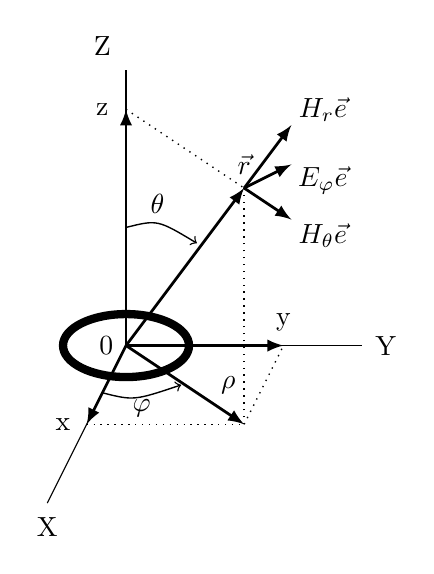
\begin{tikzpicture}
	\draw (4,4) -- (3,2)node at (3, 1.7) {X};%Fadenkreuz x
	\draw (4,4) node at(3.75,4) {0} -- (7,4)node at (7.3, 4) {Y};%Fadenkreuz y
	\draw (4,4) -- (4,7.5)node at (3.7, 7.8) {Z};%Fadenkreuz z
	
	\draw[line width=1pt, ->, >=latex](4, 4)  -- (3.5, 3) node at (3.2, 3) {x};
	\draw[line width=1pt, ->, >=latex](4, 4)  -- (6, 4) node at (6, 4.3) {y};
	\draw[line width=1pt, ->, >=latex](4, 4)  -- (4, 7) node at (3.7, 7) {z};
	
	\draw[line width=0.5pt, style=dotted](3.5, 3) -- (5.5, 3);%Projektion y Rcihtung
	\draw[line width=0.5pt, style=dotted](5.5, 3) -- (6, 4);%Projektion x Rcihtung
	
	\draw[line width=1pt, ->, >=latex](4, 4)  -- (5.5, 3) node at (5.3, 3.5) {$\rho$};
	
	\draw[line width=1pt, ->, >=latex](4, 4)  -- (5.5, 6) node at (5.5, 6.3) {$\vec{r}$};
	
	\draw[line width=0.5pt, style=dotted](5.5, 3) -- (5.5, 6);%Projektion p zu \vec{r}
	\draw[line width=0.5pt, style=dotted](4, 7) -- (5.5, 6);%Projektion von z zur \vec{r}
	
	\coordinate (A) at (4, 5.5);
	\coordinate (B) at (4.9, 5.3);
	\coordinate (a) at (4.4, 5.6);
	\draw[line width=0.5pt, cap=round,->](A) .. controls (a) .. (B) node at (4.4, 5.8){$\theta$};
	
	\coordinate (C) at (3.7, 3.4);
	\coordinate (D) at (4.7, 3.5);
	\coordinate (c) at (4.1, 3.3);
	\draw[line width=0.5pt, cap=round,->](C) .. controls (c) .. (D) node at (4.2, 3.2){$\varphi$};
	
	%Einheitsvektoren
	\draw[line width=1pt, ->, >=latex](5.5, 6)  -- (6.1, 6.8) node at (6.5, 7) {$H_{r}\vec{e}$};
	\draw[line width=1pt, ->, >=latex](5.5, 6)  -- (6.1, 5.6) node at (6.5, 5.4) {$H_{\theta}\vec{e}$};
	\draw[line width=1pt, ->, >=latex](5.5, 6)  -- (6.1, 6.3) node at (6.5, 6.1) {$E_{\varphi} \vec{e}$};
	
	%Antenne Loop
\draw[line width=3pt](4, 4) ellipse (0.8 and 0.4);
\end{tikzpicture}
\end{center}
\caption{Loop Antenne mit Feldvektor und Einheitsvektoren}
\label{LoopFerdVektor}
\end{figure}
%%%%%%%%%%%%%%%%%%%%%%%%%%%%%%%%%%%%%%%%%%%%%%%%%%%%%%%%%%%%%%%%%%%
